\documentclass[a4paper,11pt]{article}%必须以此为开头,可以在[]内设置栏数,单双面,横竖向
\usepackage{latexsym}%符号字体
\usepackage{makeidx}%制作索引
\makeindex
\usepackage{ifthen}%提供分支语句
\usepackage{ctex}%提供中文支持
\usepackage{graphicx}%用于插入图片
\usepackage{amsmath}%用于数学公式
\usepackage{IEEEtrantools}%用于使用IEEE数学公式排版工具
\usepackage{amsfonts}%用于其他字体的数学符号
\usepackage{amsthm}%提供证明,定理等环境
\usepackage{amssymb}%用于提供各种数学符号
\usepackage{mathrsfs}%用于提供花体字母
\usepackage{verbatim}%使用\verbatiminput{filename}来直接导入文件中的文本内容
\usepackage{layouts}%用于设置页面布局
\usepackage{calc}%允许一些常量参量用算术表达式代替
\author{Fan}
\title{Test}
\date{\today}
\begin{document}
\maketitle
\tableofcontents
\begin{abstract}
    The abstract 阿巴斯塔塔
\end{abstract}
\pagestyle{plain}%页面风格,plain为中下方有页码.heading是页眉中间有页数,同时有章节名,empty是空页眉页尾
%\thispagestyle{pagestyle}%本页页面风格
\section{Elementary}
%空格与换行
 每一行开头的空格会被忽略 正常位置的一个空格当然会被视为一个空格
换行会被视为一个空格   多个连续的空格也会被视为一个空格(这些对于英文有效,写中文的时候都是不产生空格的)

两行文字中间的空白行会被视为另起一段的标志,多行空白页等同于一行空白\\
$\backslash\backslash$也可以用于换行,也可以使用\newline $\backslash$ newline来另起一段\\*
$\backslash\backslash$*只是换行,不另起一段

命令后的空格会被忽略,可以通过在命令后添加\{\}再添加空格的方式来实现输出

\verb+\quad和\qquad+用于生成不同长度的空格

\verb+\phantom{text}+会产生相当于text中文本长度的空格

\textbackslash linebreak[n],nolinebreak,pagebreak,nopagebreak后面都可以跟[n],其中n为0-4,表示建议的程度

label\{marker\}会将该处进行标识,在文章其他位置处使用ref或pageref可以生产跳转至该处或该页的链接

footnote可以生成脚注
%其他

引用的单引号和双引号不是直接键盘上的符号,左边应该是\`,右边应该是\'.

dash用连续三个的减号-

波浪号是$\sim$

摄氏度的小圆圈$\circ$

省略号不是直接打三个英文句号,而是用$\ldots$

带星号的各种命令与不带星号的命令的区别在于,在其他计数或编号相关的代码执行时,前者会被忽略.

\verb+\newcommand{cmd}{def}+可以用于自定义命令,cmd中是自定义的命令,def中是对应的实际命令

\verb|\rule[lift]{width}{thickness}|可以产生一条竖直方向的黑色粗条纹,其中lift参数是指下边的起始位置.

%转义符\
\#\$\%\^\&\_\{\}\`\textbackslash 都需要通过转义符\textbackslash 来实现

\section{error handling}
\textbackslash sloppy可以用来消除overfull hbox的错误,该错误是指一行的长度超出了预定长度,该命令会强制减少该行内的字数,用fussy可以抵消效果

\section{Environment}
\begin{enumerate}
    \item 环境可以嵌套:
    \begin{itemize}
        \item 但别嵌套太多
        \item [-] 看上去有点傻
    \end{itemize}
    \item 因此:
    \begin{description}
        \item[Good] 可以用于是事物的定义
        \item[Bad] 不用于事物的定义
    \end{description}
\end{enumerate}
\begin{quote}
    一般而言一行中不应该有超过66个英文字母,这也是为什么默认的边距那么大
\end{quote}
\begin{verbatim}
    这个环境用于原样输出,也可以直接使用\verb+text+的形式来原样
    输出text,其中+用作分隔符,
    可以用出了*或者空格以外的符号来代替,不能用字母来代替
    
    下面将介绍\begin{tabular}[pos]{table spec}命令
\end{verbatim}
table spec中,可以填入lrc和p\{\}分别代表左对齐,右对齐,中间对齐和带有换行的文字
(正常情况下,在制表环境下,latex不会自动换行),除此之外用|代表竖线

pos中可以填入tb和c,用于指定表格在页面中的位置,分别代表顶部,底部和中间

在制表环境中,\&可以跳至下一列,\textbackslash\textbackslash 可以用于新起一行
\verb+\hline+用于插入水平线,\verb+\cline{i-j}+用于指定添加由i列到j列的横线

|可以用\verb+@{}+来替换,括号中间的符号会用于替换横线,如果是空白的话会把横线处留出的空格消除
如果没有在table spec中添加左右两侧的横线的话会默认预留出空格的位置

\verb+\multicolumn{2}{c}{text}+用于将多列合并,用于这些列的首行位置,
第一个括号内为合并的行数,第二个括号内为合并后对齐的方式,第三个括号内为合并后首行的内容

\begin{tabular}[c]{c | r @{.} l}
    Pi expression & \multicolumn{2}{c}{Value}\\
    \hline
    $\pi$   & 3&1416\\
    $\pi^{\pi}$ &36&46\\
    $(\pi^{\pi})^{\pi}$ & 80662 & 7\\
\end{tabular}


在multline环境中,可以对数学公式进行多行排版,与equation环境的区别在于,在该环境中
换行是可以人为控制,任意插入的,通过\textbackslash\textbackslash 来实现

在align环境中,可以通过\&来进行对齐,每一行默认进行编号,若某行无需编号,可在末尾添加\verb+nonumber+

IEEEeqnarray环境用于数学公式多行排版
\begin{verbatim}
    \begin{IEEEeqnarray}{rCl}
        a&=&b+c
        \\
        &=&d+e+f+g+h
        +i+j+k\nonumber \\
        & & \negmedspace {} +l +m+ n+ o
        \\
        & = & p+q+r+s
    \end{IEEEeqnarray}
\end{verbatim}
\begin{IEEEeqnarray}{rCl}
    a&=&b+c
    \\
    &=&d+e+f+g+h
    +i+j+k\nonumber \\
    & & \negmedspace {} +l +m+ n+ o
    \\
    & = & p+q+r+s
\end{IEEEeqnarray}

上面是一个用该环境解决连续多个加号并且需要换行的情况,其中rCL表示3列,对齐方法分别是右对齐,居中和左对齐
其中C被大写了,意味着会在该列两侧额外添加一些空格.rclRCL都是用于数学公式,
而stu则是用于文字,分别是左对齐,居中,右对齐.
额外的空格也可以通过.和/和?来添加,对应的空格长度依次增加.还可以用+来代表不定长的空格,用来占满剩余空间
\begin{verbatim}
\begin{proof}
    This is a proof that ends
    with an equation array:
    \begin{IEEEeqnarray}{+rCl+x*}
    a & = & b + c \\
    & = & d + e. \\
    &&& \qedhere\nonumber%不添加这一行的话会在证明结束符号的上方添加一行空白,这是错误的
    \end{IEEEeqnarray}
\end{proof}
\end{verbatim}
\begin{proof}
    This is a proof that ends
    with an equation array:
    \begin{IEEEeqnarray}{+rCl+x*}
    a & = & b + c \\
    & = & d + e. \\
    &&& \qedhere\nonumber
    \end{IEEEeqnarray}
\end{proof}
    

在该环境中,当某行的等号右侧的公式过长时,可能会出现公式与编号重叠的问题.
可以在出现问题的那一行末尾添加命令\verb+\IEEEeqnarraynumspace+来解决.
如果是等号左侧的公式过长,则可以在该行开头添加\verb+\IEEEeqnarraymulticol{n}{pos}+
来进行调整,该命令与\verb+\multicolumns+命令相似,第一个参数用于指定合并的列数,
第二个参数用于指定合并后的列的对齐方式

使用IEEEeqnarray*环境可以默认去除公式编号,可以通过\verb+\IEEEyesnumber+来手动添加*.*样式的编号.
也可以使用\IEEEyessubnumber 来添加*.*x样式的子编号

在上述两个环境中,如果像放置label,应该在该行的\textbackslash\textbackslash 后添加

array环境用于排版矩阵,常嵌套与equation等数学公式环境中,该环境的使用方法和tabular环境一致,
区别在于第二个参数表中只需要填写clr这几个对齐方式.矩阵两侧的括号需要手动输入,配合\verb+\left+和
\verb+\right+来实现大括号.

cases环境用于排版分段函数
\begin{verbatim}
    \begin{equation*}
        |x| =
        \begin{cases}
        -x & \text{if } x < 0,\\
        0 & \text{if } x = 0,\\
        x & \text{if } x > 0.
        \end{cases}
        \end{equation*}
\end{verbatim}

matrix系列环境则是专门用于排版矩阵的环境,分别有matrix,pmatrix,bmatrix,Bmatrix,vamatrix,Vmatrix.
其中matrix环境不自动生产括号,而接下来几个环境依次自动生成\verb-(,[,{,|和||.-在这些环境中,排版
规则和tabular环境一致

proof环境会帮忙自动生成证明字样以及证明结束的符号,可以使用qedhere命令来指定证明结束符号所在行.,否则它会单独占据一行.
\section{graph}
\verb+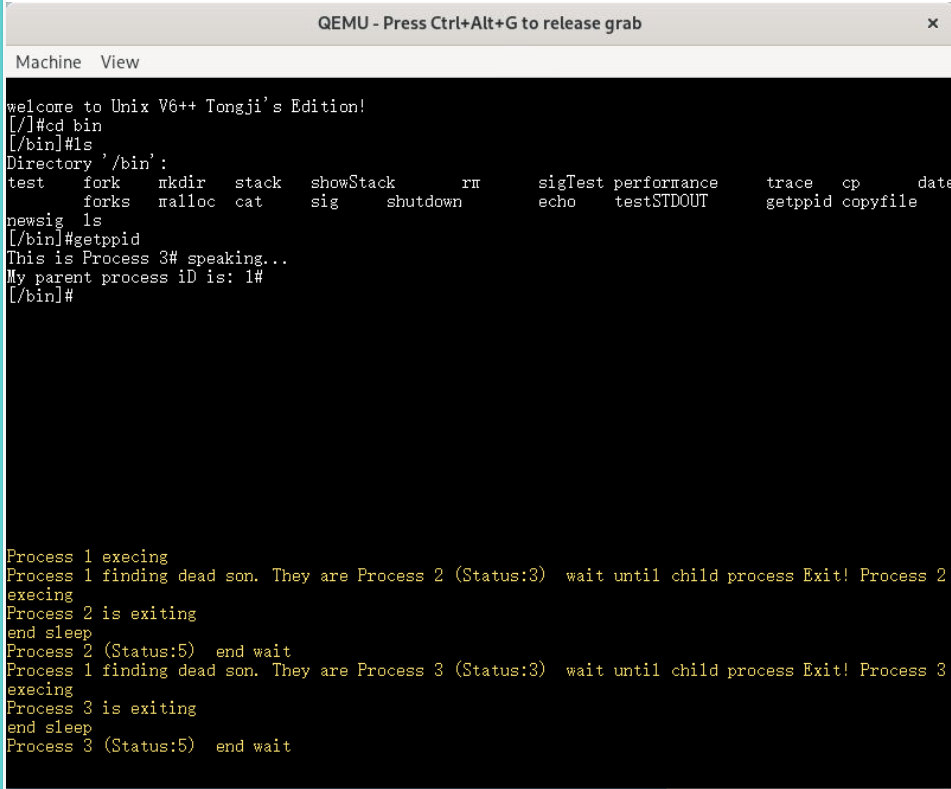
\includegraphics[angle=90,width=\textwidth,scale=1]{test.png}+

用于插入图片,
其中\verb+\textwidth+使得图片宽度和文本内容的宽度一致,当然也可以设置为其他的宽度,angle为顺时针旋转角度
scale可以用来缩放图片

\section{float}
latex为表格和图片分别提供了两种浮动体环境,分别是\\\verb+\begin{figure}[placement specifier]+和\verb+\begin{table}[P S]+

ps中可以填入htbp!,分别代表当前位置,某页的顶部,底部或者为浮动体单独开辟一页,以及强制执行这些命令.
默认为tbp

\verb+\caption[caption used in the list]{caption text}+可以为浮动体添加标题
\verb+\listoffigures和\listoftables+可以打印图片和表格的标题列表,列表中的标题为\[\]中的内容
想对浮动体进行引用的话,要在对于浮动体的\verb+\caption{}+命令的\{\}内的尾部添加\verb+\label+
\section{math}
\verb+\begin{equation}+环境用于数学公式,该环境中会将公式根据章节来进行编码,用\verb+\tag{内容}+可以取消
    该公式的编码,并用\{\}内的文字代替编码

    如果不想将公式进行编码,则使用\verb+\begin{equation*}+环境,或者在\verb+\[\]+中输入公式

在数学公式中输入文字的话要嵌套使用\verb+\text{}+

可以在前言区使用\verb+\DeclareMathOperator{指令}{对应代码}+来自定义一些数学符号

想要成对的分隔符,如括号,的大小根据其中的内容进行更改,需要在前后分隔符的前面分别添加\verb+\left+和\verb+\right+,
如果不想要其中一个分隔符,但是又想要让单独的分隔符调整大小,则在不要的分隔符用.来代替

数学公式模式中,使用\verb+\,或\:或\;或\加上空格或\quad或\qquad或\!+来产生由短到长的空格,最后一个除外.
最后一个是专门用于负号和数字之间的空格调整,是用于消去多余的间隙的

可以使用\verb+\boldsymbol{symbol}+来排版粗体符号

\subsection{theorems,lemmas,\ldots}
为了在文章中生成定理,公式,注记.需要在前言区中定义相关格式.
\begin{verbatim}
    \theoremstyle{definition/plain/remark} 
    \newtheorem{name}[counter]{text}[section]
\end{verbatim}
其中style需三选一,definition为宽罗马字体,plain为宽意大利斜体,remark为斜罗马字体.
调用自定义的格式的格式为\verb+\begin{name}[text]+和\verb+\end{name}+.
以上内容中方括号内的参数是可选的.
name是所自定义的格式的名称,counter在前言区中填入的是和该name属于同一类的name,编码时两者会视为同一个,
在使用时填入的是具体的内容,如具体的某部法律的名称.会在text后打印在括号中
text中则是会打印出来的抬头,如"定义".
在前言区若添加了section参数,会使得该格式的编码会结合该section来呈现,也可以替换为chapter或subsection关键词.

\section{引用}
\subsection{文本内相互引用}
如果想在文本内相互引用,首先需要在被引用的地方插入marker,插入方法是使用指令\verb+\bibitem[label]{marker}+,
引用处插入指令\verb+\cite{marker}+.如果没有使用label关键词,则会自动编号.

使用案例是
\begin{verbatim}
    Partl~\cite{pa} has
proposed that \ldots
\begin{thebibliography}{99}%99指的是引用条目前的编号的长度不会超过99这个文本的长度
\bibitem{pa} H.~Partl:
\emph{German \TeX},
TUGboat Volume~9, Issue~1 (1988)
\end{thebibliography}
\end{verbatim}
Partl~\cite{pa} has
proposed that \ldots
\begin{thebibliography}{99}
\bibitem{pa} H.~Partl:
\emph{German \TeX},
TUGboat Volume~9, Issue~1 (1988)
\end{thebibliography}
\section{index 索引}
索引的指令为\verb+\index{key@formatted_entry}+.其中key是用于索引分类的,而entry是索引的关键词.
entry是可选的,如果缺失,key将会被使用.一般entry是呈现在索引表上的关键词,如果没有,则用key代替,key和entry之间加!说明该索引是该key下的子索引.
如果想对索引表中的页码进行排版,则将@entry改为|加上格式.

在想要打印索引表的地方使用命令\verb+\printindex+

\section{自定义}
\subsection{newcommand}
可以通过命令\verb+\newcommand{name}[num]{def}+来自定义指令,其中num默认为0,代表的是自定义的命令所需要的参数的数量,
如果不为零,则在def中使用\verb+#1,#2..+来代表各参数的占位符.

可以用命令\verb+\renewcommand+来覆盖之前定义的同名自定义指令,其各参数与命令\verb+\newcommand+一致.
\subsection{new environment}
可以使用命令\verb+\newenvironment{name}[num]{before}{after}+来自定义环境.num的含义与使用方法与自定义命令一致.
before与after参数分别是该自定义环境中的填写的命令之前与之后发生的命令.同样地,也有\verb+\renewenvironment+命令.

\section{字体}
\begin{table}[htp]
       \caption{Fonts}    
\begin{tabular}{llcll}
\hline
    \verb+\textrm{text}+ & \textrm{roman} &\quad & \verb+\textsf{text}+ & \textsf{sans serif} \\
    \verb+\texttt{text}+ & \texttt{typewriter} &\quad &  & \\
    \verb+\textmd{text}+ & \textmd{medium} &\quad & \verb+\textbf{text}+ & \textbf{bold face} \\
    \verb+\textup{text}+ & \textup{upright} &\quad & \verb+\textit{text}+ & \textit{italic} \\
    \verb+\textsl{text}+ & \textsl{slanted} &\quad & \verb+\textsc{text}+ & \textsc{small Caps} \\
    \verb+\emph{text}+ & \emph{emphasized} &\quad & \verb+\textnormal{text}+ & \textnormal{document font} \\
    \hline

\end{tabular}
\caption{Font Sizes}
\begin{tabular}{llcll}
    \hline
    \verb+\tiny+ & \tiny{tiny font} & \quad & \verb+\Large+ & \Large{larger font} \\
    \verb+\scriptsize+ & \scriptsize{very small font} & \quad & \verb+\LARGE+ & \LARGE{very large font} \\
    \verb+\footnotesize+ & \footnotesize{quite small font} & \quad & \verb+\huge+ & \huge{huge} \\
    \verb+\small+ & \small{small font} & \quad &  &  \\
    \verb+\normalsize+ & \normalsize{normal font} & \quad & \verb+\Huge+ & \Huge{largest} \\
    \hline
\end{tabular}
\caption{Absolute Point Sizes in Standard Classes}
\begin{tabular}{lrrr}
    \hline 
    \multicolumn{1}{c}{size} & 10pt(default) & 11pt option & 12pt option \\
    \verb+\tiny+ & 5pt & 6pt & 6pt \\
    \verb|\scriptsize| & 7pt & 8pt & 8pt \\
    \verb|footnotesize| & 8pt & 9pt & 10pt \\
    \verb|\small| & 9pt & 10pt & 11pt \\
    \verb|\normalsize| & 10pt & 11pt &12pt \\
    \verb|\large| & 12pt & 12pt & 14pt \\
    \verb|\Large| &14pt &14pt & 17pt \\
    \verb|\LARGE| & 17pt & 17pt & 20pt \\
    \verb|\huge| & 20pt & 20pt &25pt    \\
    \verb|\Huge| & 25pt & 25pt & 25pt\\
    \hline
\end{tabular}
\caption{Math Fonts}
\begin{tabular}{ll}
\hline
\verb|\mathrm{text}| & $\mathrm{Roman Font}$ \\
\verb|\mathbf{text}| & $\mathbf{Boldface Font}$ \\
\verb|\mathsf{text}| & $\mathsf{Sans Serif Font} $\\
\verb|\mathtt{text}| & $\mathtt{Typewriter Font}$ \\
\verb|\mathit{text}| & $\mathit{Italic Font}$ \\
\verb|\mathcal{text}| &$ \mathcal{Calligraphic Font}$ \\
\verb|\mathnormal{text}| & $\mathnormal{Normal Font} $\\
\hline
\end{tabular}
\end{table}
想打印特定字号的字体,可以调用同名的环境,也可以直接在同一个花括号内,以字体命令开头,然后输入文字.

\verb|\emph{text}|的强调效果会根据上下文的字体状态进行调整
\section{间距}
\subsection{行间距}
可以使用命令\verb|\linespread{factor}|来调整行间距.当factor=1.3时,为一行半,为1.6时为双倍.默认为1

更正规的命令为\verb|\setlength{\baselineskip}{1.5\baselineskip}|,案例为
\begin{verbatim}
    {\setlength{\baselineskip}%
{1.5\baselineskip}
This paragraph is typeset with
the baseline skip set to 1.5 of
what it was before. Note the par
command at the end of the
paragraph.\par}%只有当\par命令在花括号内部时,才会对于行间距才会产生调整,
当字体改变时,也只有加上\par,行间距才会随字体改变
This paragraph has a clear
purpose, it shows that after the
curly brace has been closed,
everything is back to normal.
\end{verbatim}
{\setlength{\baselineskip}%
{1.5\baselineskip}
This paragraph is typeset with
the baseline skip set to 1.5 of
what it was before. Note the par
command at the end of the
paragraph.\par}
This paragraph has a clear
purpose, it shows that after the
curly brace has been closed,
everything is back to normal.

\subsection{段间距}
段间距可以在前言区调整.
\begin{verbatim}
    \setlength{\parindent}{0pt}
    \setlength{\parskip}{1ex plus 0.5ex minus 0.2ex}
\end{verbatim}
这段指令将段落缩进设为0.skip设定的是段落之间的空格,plus和minus设定的上下浮动的范围以供调整.
为了避免对目录产生影响,可以将制作目录的命令放在该命令之前.

可以通过使用indent指令来缩进未缩进的段落,需要放在段落开头.类似的,也有noindent指令.
\subsection{其他间距}
可以分别使用hspace和vspace来调整横向和纵向的间距,常用长度单位有mm,cm,in,pt,em,ex.
特别地,stretch\{n\}会自动填充空格,直到充满整行或整页,若同时有多个stretch,会按照n参数按比例分配.
带*的hspace和vspace命令在发生换行或换页的情况时仍会保留未输入的空格.

若仍需额外调整行间距,可以使用\verb|\\[length]|.同时也有\verb|\bigskip|和\verb|\smallskip|.
\section{页面设置}
可以在前言区来设置页面的布局.可以使用\verb|\setlength{parameter}{length}|
或者\verb|\addtolength{parameter}{length}|,第一个命令时设定某参数的固定值,而第二个命令是在某参数的固定值的基础上进行增加.
各参数及其含义可以查看Ishort.pdf的115页.

可以使用命令\verb|\parbox[position]{width}{text}|或者\verb|\begin{minipage}[position]{width}text\end{minipage}|来生成
一段在框内的文字.两者的区别在于后者更加功能强大,可以在该环境中使用几乎所有命令.

\end{document}

